\documentclass[12pt,reqno]{semhas-tesis-filkom}

\title{JUDUL Tidak mengandung Spesial Karakter/Simbol\\Subtitle jika ada}

\author{%
\begin{tabular}{c} 
  \theauthor{Sunama Mahasiswa, Nama Pembimbing Pertama}
  \aff{
    Departemen Teknik Informatika\\
    Fakultas Ilmu Komputer \\
    Universitas Brawijaya \\
    Malang, Indonesia \\
    e-mail: name@student.ub.ac.id, pembimbing@ub.ac.id
    } 
\end{tabular}
\and
\begin{tabular}{c} 
  \theauthor{Nama Pembimbing Lain}
  \aff{
    Departemen Sistem Informasi \\
    Fakultas Ilmu Komputer \\
    Universitas Brawijaya \\
    Malang, Indonesia \\
    e-mail: name@ub.ac.id
    }
\end{tabular} 
% \and
% \begin{tabular}{c} 
%   \theauthor{Pembimbing Juga}
%   \aff{
%     Departemen Teknik Informatika \\
%     Fakultas Ilmu Komputer \\
%     Universitas Brawijaya \\
%     Malang, Indonesia \\
%     e-mail: name@ub.ac.id
%     }
% \end{tabular}
}

\makeatletter
\let\newtitle\@title
\let\newauthor\@author
\let\newdate\@date
\makeatother
\makeatletter
\def\and{
  \end{tabular}
  \hskip 0em
  \begin{tabular}[t]{c}}
\makeatother

\begin{document}

\maketitle
\abstrak{Abstrak adalah uraian singkat (umumnya 200-300
kata) yang merupakan intisari dari sebuah Tesis. Dalam
abstrak tidak diperkenankan mengandung special karakter,
symbol dan persamaan. Ukuran font untuk abstrak adalah 9
dan dicetak tebal (bold).}

\section{Introduction}

Makalah seminar hasil ditulis menggunakan bahasa
Indonesia yang baku.Makalah ditulis mengikuti template,
dalam format 2 kolom menggunakan kertas A4. Font yang
digunakan adalah Times New Roman. Untuk isi memiliki
ukuran font 10.

\section{Penomoran}

Penomoran untuk setiap section menggunakan angka
romawi dan dicetak tebal dengan ukuran Font 11.

\subsection{Subsection (Heading 2)}

Penomoran untuk subsection menggunakan abjad kapital
yang kemudian diikuti dengan titik dan dicetak miring
dengan font 11 begitu juga dengan judul dari subsection
dicetak miring.

\begin{equation}
  x^n + y^n = z^n
\end{equation}

Untuk equation diberikan penomeran secara urut dan nomor
berada didalam kurung. Posisi dari penomoran berada
disebelah kanan (rata kanan). Persamaan diusahakan ditulis
dalam satu baris, namun jika tidak memungkinkan dan harus
lebih dari satu baris, penomorannya diletakkan pada baris
terakhir.

\subsection{Penulisan tabel dan gambar}

Judul tabel ditulis dibagian atas tabel dengan besar font 10, sedangkan font yang digunakan didalam tabel adalah 8. Nomor tabel diberikan secara urut dan diakhiri dengan titik. Tulisan tabel menggunakan huruf besar semua seperti yang diperlihatkan pada TABEL \ref{tab:contoh}.

\begin{table}[ht]
\caption{Contoh Tabel}
\renewcommand{\arraystretch}{1.5}
\footnotesize
\newcolumntype{C}{>{\Centering\arraybackslash}X}
\begin{tabularx}{\columnwidth}{|l|l|l|l|}
  \hline
  % \toprule
  \multirow{2}{*}{\textbf{Table Head}} & \multicolumn{3}{c|}{\textbf{Table Column Head}} \\
  \cline{2-4}
  % \multirow{3}{4em}{Multiple row} & cell2 & cell3 \\ 
  & \multicolumn{1}{C|}{\bfseries\itshape{Table column subhead}} & \bfseries\itshape{Subhead} & \bfseries\itshape{Subhead} \\ 
  \hline
  cell8 & cell9 & cell & cell \\ 
  cell8 & cell9 & cell & cell \\
  cell8 & cell9 & cell & cell \\
  cell8 & cell9 & cell & cell \\
  \hline
\end{tabularx}
\label{tab:contoh}
\end{table}

Untuk judul gambar dan grafik diletakkan dibagian bawah
gambar/grafik dengan ukuran font 10 \cite{bookseries,collection}. Posisi Gambar berada
ditengah. Jika terdapat gambar lebih dari satu dalam sebuah
judul Gambar, maka dapat ditempatkan sedemikian rupa
dari kiri ke kanan atau atas bawah. Setiap Gambar diberi
penomoran dengan abjad dan diberi kurung (a). Sitasi:.\cite{anggariawan:2014}, \cite{Bloggs1950}, \cite{abook,acceptedpub,anarticle}

\begin{figure}[ht]
  \centering
  \begin{subfigure}[h]{\columnwidth}
    \centering
  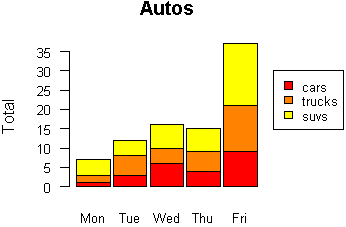
\includegraphics[width=0.6\columnwidth]{babs/images/bar_script4.png}
  \subcaption{Grafik 1}
  \vspace*{1em}
  \end{subfigure}
  \begin{subfigure}[h]{\columnwidth}
    \centering
    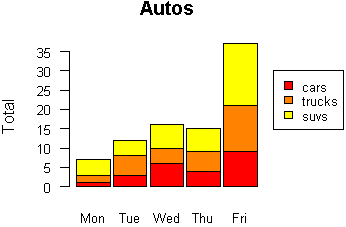
\includegraphics[width=0.6\columnwidth]{babs/images/bar_script4.png}
  \subcaption{Grafik 2}
  \end{subfigure}
  \caption{Contoh Penulisan Grafik yang Memiliki
  Katagori Sama. (a) Grafik1 dan (b) Grafik 2}
\end{figure}

\subsection{Penulisan satuan}

Penulisan satuan dalam makalah seminar Tesis ini
menggunakan standar internasional SI atau CGS. Satuan
ditulis dalam unit yang sama seperti "Wb/m\textsuperscript{2}" bukan
"Weber/m\textsuperscript{2}". Pengejaan satuan hanya dapat dilakukan di dalam kalimat. Penulisan bilangan desimal pecahan harus ditambah nol sebelum titik “0.25” bukan ”.25”. \cite{conv,notpub,report,thesis,unpub,website}

\subsection{Referensi}

Penulisan referensi menggunakan font dengan ukuran 9 dan diberikan penomoran secara urut sesuai dengan urutan sitasinya didalam paper serta diberi kurung kotak. Sitasi dari referensi didalam kalimat, cukup dengan menuliskan nomor urutnya saja [1]. Jika sebelumnya referensi telah pernah diacu, dan kemudian diacu pada kalimat berikutnya dengan referensi yang lebih dari satu dan acak maka semua nomor referensi harus dituliskan. Sebagai contoh [1],[3],[5] yang artinya mensitasi referensi nomor urut 1, 3 dan 5. Jika yang disitasi referensi adalah urut maka dapat dituliskan [1]-[6] yang artinya mensitasi referensi dari nomor 1 sampai dengan nomor 6.

\section*{Ucapan Terima Kasih}

Sebelum referensi dapat juga ditambah dengan ucapan
terimakasih kepada pihak-pihak yang telah mendukung
terselesainya penelitian tersebut.

\vspace*{1em}
\balance

\renewcommand{\refname}{\centering\NoCaseChange\itshape{Referensi}\vspace*{1em}}

\bibliographystyle{IEEEtran}
\bibliography{referensi}

\end{document}